%% talk5.tex
%% Copyright 2022 Tom M. Ragonneau
%
% This work may be distributed and/or modified under the
% conditions of the LaTeX Project Public License, either version 1.3
% of this license or (at your option) any later version.
% The latest version of this license is in
%   http://www.latex-project.org/lppl.txt
% and version 1.3 or later is part of all distributions of LaTeX
% version 2005/12/01 or later.
%
% This work has the LPPL maintenance status `maintained'.
%
% The Current Maintainer of this work is Tom M. Ragonneau.
\documentclass{polyu-presentation}  % handout
\usepackage{microtype}
\usepackage{booktabs}

% List of hyphenation exceptions for US English
% Source: https://ctan.org/tex-archive/info/digests/tugboat/hyphenex
\input{ushyphex}

% Bibliographical resources
\addbibresource{ragonneau-bib/strings.bib}
\addbibresource{ragonneau-bib/optim.bib}

% Dedicated mathematical macros
\newcommand{\con}[1]{c_{#1}}
\newcommand{\conm}[2][]{\hat{c}_{#2}\ifthenelse{\equal{#1}{}}{}{^{#1}}}
\newcommand{\ieq}{\mathcal{E}}
\newcommand{\iub}{\mathcal{I}}
\newcommand{\lag}{\mathcal{L}}
\newcommand{\lagm}[1][]{\hat{\mathcal{L}}\ifthenelse{\equal{#1}{}}{}{^{#1}}}
\newcommand{\merit}[1][]{\varphi\ifthenelse{\equal{#1}{}}{}{^{#1}}}
\newcommand{\meritm}[1][]{\hat{\varphi}\ifthenelse{\equal{#1}{}}{}{^{#1}}}
\newcommand{\obj}{f}
\newcommand{\objm}[1][]{\hat{f}\ifthenelse{\equal{#1}{}}{}{^{#1}}}
\newcommand{\qpoly}{\mathscr{Q}(\R^n)}
\newcommand{\ratio}[1][]{\rho\ifthenelse{\equal{#1}{}}{}{^{#1}}}
\newcommand{\xl}{l}
\newcommand{\xpt}[1][]{\mathcal{Y}\ifthenelse{\equal{#1}{}}{}{^{#1}}}
\newcommand{\xu}{u}

% Performance and data profiles
\usepackage{xstring}
\newcommand{\drawprofiles}[4]{%
    \def\selectsolvers{#2}%
    \def\selectcsv{figures/#3}%
    \def\selectprofile{#4}%
    \ifthenelse{\equal{#1}{performance}}{%
        \def\selectxlabel{$\log_2(\alpha)$}%
        \def\selectylabel{Performance profiles~$\rho_s(\alpha)$}%
    }{%
        \def\selectxlabel{Number of simplex gradients~$\alpha$}%
        \def\selectylabel{Data profiles~$d_s(\alpha)$}%
    }
    %% utils/profiles.tex
%% Copyright 2022 Tom M. Ragonneau
%
% This work may be distributed and/or modified under the
% conditions of the LaTeX Project Public License, either version 1.3
% of this license or (at your option) any later version.
% The latest version of this license is in
%   http://www.latex-project.org/lppl.txt
% and version 1.3 or later is part of all distributions of LaTeX
% version 2005/12/01 or later.
%
% This work has the LPPL maintenance status `maintained'.
%
% The Current Maintainer of this work is Tom M. Ragonneau.
\begin{tikzpicture}[scale=0.9]
    \pgfplotstableread[col sep=comma]{\selectcsv}\selectcsvread
    \newcommand{\getxmaxcsv}[1]{%
        \pgfplotstablegetrowsof{\selectcsvread}%
        \pgfmathtruncatemacro{\LastRowNo}{\pgfplotsretval-1}%
        \pgfplotstablesort[sort key={#1}]{\csvsorted}{\selectcsvread}%
        \pgfplotstablegetelem{\LastRowNo}{#1}\of{\csvsorted}%
        \pgfmathsetmacro{\selectxmaxcsv}{\pgfplotsretval}%
    }
    \pgfmathparse{\selectsolvers[0]}
    \let\selectsolver\pgfmathresult\relax
    \getxmaxcsv{x\selectprofile_\selectsolver}
    \begin{axis}[%
        width=205pt,%
        xmin=0,%
        xmax=0.55*\selectxmaxcsv,%
        ymin=0,%
        ymax=1,%
        minor y tick num=1,%
        yminorticks=true,%
        ytick={0,0.2,...,1},%
        cycle list name=profiles,%
        legend pos=south east,%
        xlabel={\selectxlabel},%
        ylabel={\selectylabel},%
        xticklabel style={/pgf/number format/1000 sep={}},%
    ]
        \pgfmathparse{dim{\selectsolvers}-1}
        \let\selectlastindex\pgfmathresult\relax
        \foreach \i in {0,1,...,\selectlastindex} {%
            \pgfmathparse{\selectsolvers[\i]}%
            \let\selectsolver\pgfmathresult\relax%
            \StrSubstitute{\selectsolver}{-}{~}[\selectsolverescaped]%
            \addplot table[%
            x=x\selectprofile_\selectsolver,%
            y=y\selectprofile,%
            col sep=comma,%
            ]{\selectcsvread};%
            \addlegendentryexpanded{\selectsolverescaped}%
        }
    \end{axis}
\end{tikzpicture}%
}
\newcommand{\drawperformanceprofiles}[3]{\drawprofiles{performance}{#1}{#2}{#3}}
\newcommand{\drawdataprofiles}[3]{\drawprofiles{data}{#1}{#2}{#3}}

\title{Model-Based DFO Methods and Software}
\subtitle[The COBYQA Method]{Talk no.\ 5 \textemdash\ The COBYQA Method}
\author[Tom M. Ragonneau]{\texorpdfstring{
    Tom M. Ragonneau\\ 
    \footnotesize Co-supervised by Dr.\ Zaikun Zhang and by Prof.\ Xiaojun Chen
}{Tom M. Ragonneau}}
\institute[PolyU AMA]{
    Department of Applied Mathematics\\
    The Hong Kong Polytechnic University
}
\date{November 23, 2022}
\titlegraphic{}

\begin{document}

\begin{frame}
	\titlepage
\end{frame}

\begin{frame}
    \frametitle{Table of contents}

	\tableofcontents[hideallsubsections]
\end{frame}

\section{Introduction and motivation}

\begin{frame}
    \frametitle{The problem}

	We design a \alert{method} to solve
    \begin{align*}
        \min_{x \in \R^n}   & \quad \obj(x)\\
        \text{s.t.}         & \quad \con{i}(x) \le 0, ~ i \in \iub,\\
                            & \quad \con{i}(x) = 0, ~ i \in \ieq,\\
                            & \quad \xl \le x \le \xu,
    \end{align*}
    where \alert{derivatives} of~$\obj$ and~$\con{i}$ are \alert{unknown}.

    \medskip

    \begin{block}{}
        We assume that the bound constraints~$\xl \le x \le \xu$ are \alert{inviolable}.
        \begin{enumerate}[<+(1)->]
            \item $f$ and/or~$\con{i}$ may \alert{not} be defined otherwise.
            \item The algorithm \alert{must always respect} the bound constraints.
        \end{enumerate}
    \end{block}
\end{frame}

\begin{frame}
    \frametitle{The hyperparameter tuning of an SVM}

    A \alert{binary SVM classifier}~$\delta(x) = \sgn(\beta + \omega^{\T} \psi(x))$ can be obtained by solving
    \begin{align*}
        \min_{(\omega, \beta, \xi) \in \R^{\ell} \times \R \times \R^m} & \quad\frac{1}{2} \norm{\omega}_2^2 + C \norm{\xi}_1\\
        \text{s.t.}                                                     & \quad y_i (\beta + \omega^{\T} \psi(x_i)) \ge 1 - \xi_i, ~ i = 1, 2, \dots, m,\\
                                                                        & \quad \xi \ge 0,
    \end{align*}
    for a \alert{training dataset}~$\set{(x_i, y_i)}_{i = 1}^m \subseteq \R^n \times \set{\pm 1}$ and some~$\psi : \R^n \to \R^{\ell}$.

    \medskip

    \begin{block}{Hyperparameter tuning problem}
        Given a \alert{testing dataset}, what is the \alert{best}~$C$ for this classification problem?
        \begin{enumerate}[<+(1)->]
            \item The problem is well-defined \alert{only if}~$C > 0$.
            \item In practice,~$\psi$ also depends on several \alert{parameters}.
            \item Hyperparameter tuning problems are usually \alert{DFO problems}.
        \end{enumerate}
    \end{block}
\end{frame}

\section{The derivative-free trust-region SQP method}

% Derivative-free trust-region SQP framework
% Lagrange multiplier approximation
% Trust-region radius
% Geometry-improvement
% Merit function and penalty parameter

\begin{frame}
    \frametitle{Initial design of COBYQA}

	We want to entertain the \alert{trust-region SQP} iterations
    \begin{empheq}[left={x^{k + 1} = \empheqlbrace}]{alignat*=2}
        & x^k + d^k     && \quad \text{if~$\merit(x^k + d^k) < \merit(x^k)$,}\\
        & x^k           && \quad \text{otherwise,}
    \end{empheq}
    given a \alert{merit function}~$\merit$, where the \alert{trial step}~$d^k$ approximately solves
    \begin{align*}
        \min_{d \in \R^n}   & \quad \textcolor<2->{Orange}{\nabla \obj}(x^k)^{\T} d + \frac{1}{2} d^{\T} \textcolor<2->{Orange}{\nabla_{x, x}^2 \lag}(x^k, \lambda^k) d\\
        \text{s.t.}         & \quad \con{i}(x^k) + \textcolor<2->{Orange}{\nabla \con{i}}(x^k)^{\T} d \le 0, ~ i \in \iub,\\
                            & \quad \con{i}(x^k) + \textcolor<2->{Orange}{\nabla \con{i}}(x^k)^{\T} d = 0, ~ i \in \ieq,\\
                            & \quad \xl \le x^k + d \le \xu,\\
                            & \quad \norm{d} \le \Delta^k,
    \end{align*}
    for some~$\lambda^k$ and some~$\Delta^k > 0$.
    \only<2->{\textcolor{Orange}{\textbf{But the derivatives are unknown\dots}}}
\end{frame}

\begin{frame}
    \frametitle{Interpolation-based quadratic models}

    We \alert{replace}~$\obj$ by a \alert{quadratic model}~$\objm[k]$ obtained by \alert{interpolation} on~$\xpt[k] \subseteq \R^n$.

    \medskip

    \begin{block}{Derivative-free symmetric Broyden update}
        We \alert{fix}~$n + 2 \le \card(\xpt[k]) \le (n + 1)(n + 2) / 2$ and let~$\objm[k]$ solve
        \begin{align*}
            \min_{Q \in \qpoly} & \quad \norm{\nabla^2 Q - \nabla^2 \objm[k - 1]}_{\mathsf{F}}\\
            \text{s.t.}         & \quad Q(y) = \obj(y), ~ y \in \xpt[k],
        \end{align*}
        with~$\objm[-1] \equiv 0$.
        By \alert{default}, we choose~$\card(\xpt[k]) = 2n + 1$.
    \end{block}

    \medskip

    The \alert{same calculations} are made for~$\set{\conm[k]{i}}_{i \in \iub \cup \ieq}$.

    \medskip

    \begin{block}{Hence the name}
        \alert{C}onstrained \alert{O}ptimization \alert{BY} \alert{Q}uadratic \alert{A}pproximations (\alert{COBYQA}).
    \end{block}
\end{frame}

\begin{frame}
    \frametitle{The derivative-free trust-region SQP iterations}

    The \alert{trial step}~$d^k$ approximately solves
    \begin{align*}
        \min_{d \in \R^n}   & \quad \textcolor{Orange}{\nabla \objm[k]}(x^k)^{\T} d + \frac{1}{2} d^{\T} \textcolor{Orange}{\nabla_{x, x}^2 \lagm[k]}(x^k, \lambda^k) d\\
        \text{s.t.}         & \quad \con{i}(x^k) + \textcolor{Orange}{\nabla \conm[k]{i}}(x^k)^{\T} d \le 0, ~ i \in \iub,\\
                            & \quad \con{i}(x^k) + \textcolor{Orange}{\nabla \conm[k]{i}}(x^k)^{\T} d = 0, ~ i \in \ieq,\\
                            & \quad \xl \le x^k + d \le \xu,\\
                            & \quad \norm{d} \le \Delta^k,
    \end{align*}
    and we set~$\xpt[k + 1] = (\xpt[k] \setminus \set{\bar{y}}) \cup \set{x^k + d^k}$ for some~$\bar{y} \in \xpt[k]$.

    \begin{block}{Many questions must be addressed}
        \begin{enumerate}[<+(1)->]
            \item What if the SQP subproblem is \alert{infeasible}?
            \item How to \alert{calculate}~$\lambda^k$ and~$\Delta^k$? Using what \alert{merit function}?
            \item What if~$\xpt[k]$ is almost \alert{nonpoised}?
        \end{enumerate}
    \end{block}
\end{frame}

\begin{frame}
    \frametitle{What if the subproblem is infeasible?}

    We employ a \alert{Byrd-Omojokun} approach~$d^k = n^k + t^k$.

    \medskip

    \begin{columns}
        \begin{column}{0.5\textwidth}
	        \begin{center}
                \only<1>{%
                    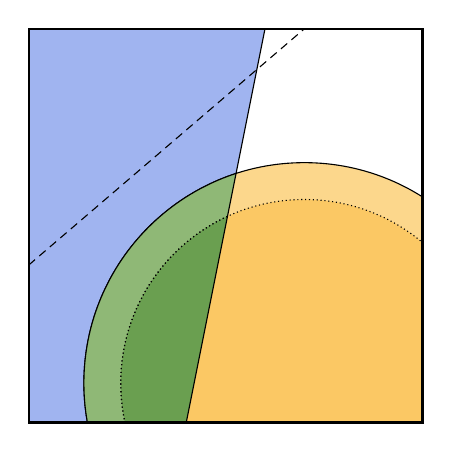
\begin{tikzpicture}
                        \fill [color=RoyalBlue!50] (0,-3) -- (1,2) -- (-2,2) -- (-2,-3) -- cycle;
                        \begin{scope}
                            \clip (-2,-3) rectangle (3,2);
                            \draw[fill=Dandelion!50] (1.5,-2.5) circle (2.8);
                            \draw[densely dotted,fill=Dandelion!70] (1.5,-2.5) circle (2.332002);
                        \end{scope}
                        \begin{scope}
                            \clip (0,-3) -- (1,2) -- (-2,2) -- (-2,-3) -- cycle;
                            \draw[fill=OliveGreen!50] (1.5,-2.5) circle (2.8);
                            \draw[densely dotted,fill=OliveGreen!70] (1.5,-2.5) circle (2.332002);
                            \draw[densely dotted] (1.5,-2.5) circle (2.332002);
                        \end{scope}
                        \draw (0,-3) -- (1,2);
                        \draw[densely dashed] (-2,-1) -- (1.5,2);
                        % \draw[densely dashed] (-2,-17/7) -- (3,13/7);
                        \draw[thick] (-2,-3) rectangle (3,2);
                    \end{tikzpicture}%
                }%
                \only<2>{%
                    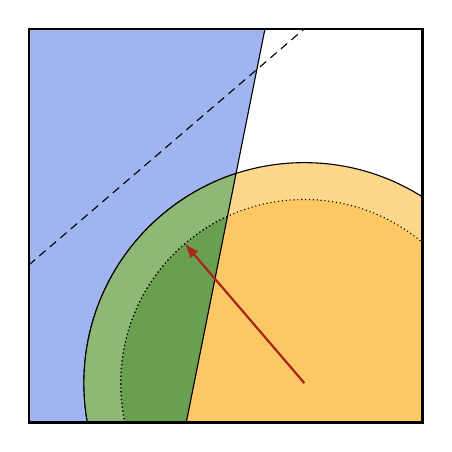
\begin{tikzpicture}
                        \fill [color=RoyalBlue!50] (0,-3) -- (1,2) -- (-2,2) -- (-2,-3) -- cycle;
                        \begin{scope}
                            \clip (-2,-3) rectangle (3,2);
                            \draw[fill=Dandelion!50] (1.5,-2.5) circle (2.8);
                            \draw[densely dotted,fill=Dandelion!70] (1.5,-2.5) circle (2.332002);
                        \end{scope}
                        \begin{scope}
                            \clip (0,-3) -- (1,2) -- (-2,2) -- (-2,-3) -- cycle;
                            \draw[fill=OliveGreen!50] (1.5,-2.5) circle (2.8);
                            \draw[densely dotted,fill=OliveGreen!70] (1.5,-2.5) circle (2.332002);
                            \draw[densely dotted] (1.5,-2.5) circle (2.332002);
                        \end{scope}
                        \draw (0,-3) -- (1,2);
                        \draw[densely dashed] (-2,-1) -- (1.5,2);
                        % \draw[densely dashed] (-2,-17/7) -- (3,13/7);
                        \draw[thick] (-2,-3) rectangle (3,2);
    
                        \draw[thick,-latex,Mahogany] (1.5,-2.5) -- (-3/170,-62/85);
                    \end{tikzpicture}%
                }%
                \only<3>{%
                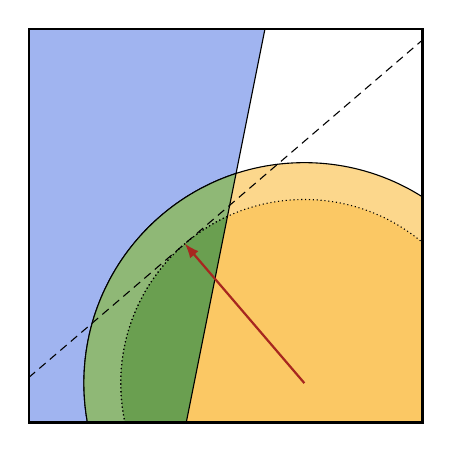
\begin{tikzpicture}
                    \fill [color=RoyalBlue!50] (0,-3) -- (1,2) -- (-2,2) -- (-2,-3) -- cycle;
                    \begin{scope}
                        \clip (-2,-3) rectangle (3,2);
                        \draw[fill=Dandelion!50] (1.5,-2.5) circle (2.8);
                        \draw[densely dotted,fill=Dandelion!70] (1.5,-2.5) circle (2.332002);
                    \end{scope}
                    \begin{scope}
                        \clip (0,-3) -- (1,2) -- (-2,2) -- (-2,-3) -- cycle;
                        \draw[fill=OliveGreen!50] (1.5,-2.5) circle (2.8);
                        \draw[densely dotted,fill=OliveGreen!70] (1.5,-2.5) circle (2.332002);
                        \draw[densely dotted] (1.5,-2.5) circle (2.332002);
                    \end{scope}
                    \draw (0,-3) -- (1,2);
                    % \draw[densely dashed] (-2,-1) -- (1.5,2);
                    \draw[densely dashed] (-2,-17/7) -- (3,13/7);
                    \draw[thick] (-2,-3) rectangle (3,2);

                    \draw[thick,-latex,Mahogany] (1.5,-2.5) -- (-3/170,-62/85);
                \end{tikzpicture}%
            }%
            \only<4>{%
            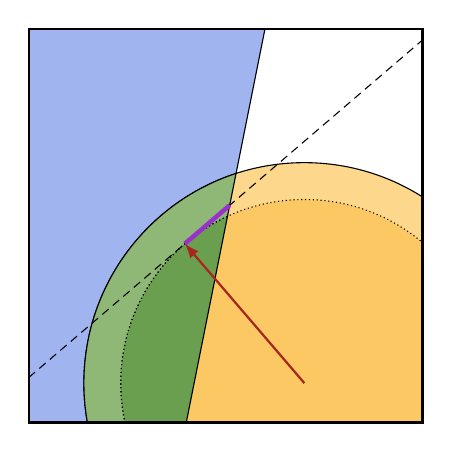
\begin{tikzpicture}
                \fill [color=RoyalBlue!50] (0,-3) -- (1,2) -- (-2,2) -- (-2,-3) -- cycle;
                \begin{scope}
                    \clip (-2,-3) rectangle (3,2);
                    \draw[fill=Dandelion!50] (1.5,-2.5) circle (2.8);
                    \draw[densely dotted,fill=Dandelion!70] (1.5,-2.5) circle (2.332002);
                \end{scope}
                \begin{scope}
                    \clip (0,-3) -- (1,2) -- (-2,2) -- (-2,-3) -- cycle;
                    \draw[fill=OliveGreen!50] (1.5,-2.5) circle (2.8);
                    \draw[densely dotted,fill=OliveGreen!70] (1.5,-2.5) circle (2.332002);
                    \draw[densely dotted] (1.5,-2.5) circle (2.332002);
                \end{scope}
                \draw (0,-3) -- (1,2);
                % \draw[densely dashed] (-2,-1) -- (1.5,2);
                \draw[densely dashed] (-2,-17/7) -- (3,13/7);
                \draw[thick] (-2,-3) rectangle (3,2);

                \draw[ultra thick,DarkOrchid] (-3/170,-62/85) -- (16/29,-7/29);
                \draw[thick,-latex,Mahogany] (1.5,-2.5) -- (-3/170,-62/85);
            \end{tikzpicture}
        }
            \end{center}
        \end{column}
        \begin{column}{0.5\textwidth}
            \only<1>{%
                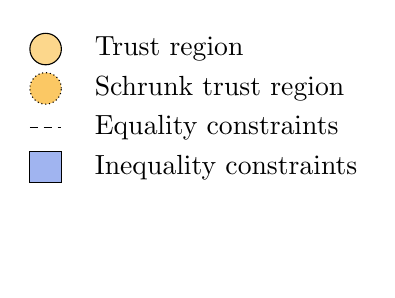
\begin{tikzpicture}
                    \draw[fill=Dandelion!50] (0,0) circle (.2);
                    \draw[densely dotted, fill=Dandelion!70] (0,-.5) circle (.2);
                    \draw[densely dashed] (-.2,-1) -- (.2,-1);
                    \draw[fill=RoyalBlue!50] (-.2,-1.7) rectangle (.2,-1.3);
                    \draw[thick,-latex,white] (-.2,-2) -- (.2,-2);
                    \draw[ultra thick,white] (-.2,-2.5) -- (.2,-2.5);
                    \node[right] at (.5,0) {Trust region};
                    \node[right] at (.5,-.5) {Schrunk trust region};
                    \node[right] at (.5,-1) {Equality constraints};
                    \node[right] at (.5,-1.5) {Inequality constraints};
                    \node[right,white] at (.5,-2) {Normal step~$n^k$};
                    \node[right,white] at (.5,-2.5) {Feasible region for~$t^k$};
                \end{tikzpicture}%
            }%
            \only<2-3>{%
                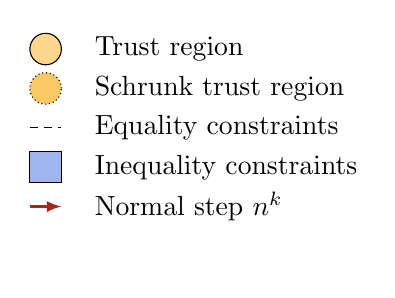
\begin{tikzpicture}
                    \draw[fill=Dandelion!50] (0,0) circle (.2);
                    \draw[densely dotted, fill=Dandelion!70] (0,-.5) circle (.2);
                    \draw[densely dashed] (-.2,-1) -- (.2,-1);
                    \draw[fill=RoyalBlue!50] (-.2,-1.7) rectangle (.2,-1.3);
                    \draw[thick,-latex,Mahogany] (-.2,-2) -- (.2,-2);
                    \draw[ultra thick,white] (-.2,-2.5) -- (.2,-2.5);
                    \node[right] at (.5,0) {Trust region};
                    \node[right] at (.5,-.5) {Schrunk trust region};
                    \node[right] at (.5,-1) {Equality constraints};
                    \node[right] at (.5,-1.5) {Inequality constraints};
                    \node[right] at (.5,-2) {Normal step~$n^k$};
                    \node[right,white] at (.5,-2.5) {Feasible region for~$t^k$};
                \end{tikzpicture}%
            }%
            \only<4>{%
            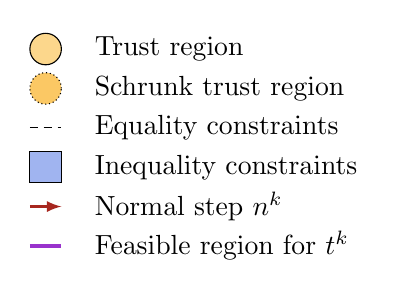
\begin{tikzpicture}
                \draw[fill=Dandelion!50] (0,0) circle (.2);
                \draw[densely dotted, fill=Dandelion!70] (0,-.5) circle (.2);
                \draw[densely dashed] (-.2,-1) -- (.2,-1);
                \draw[fill=RoyalBlue!50] (-.2,-1.7) rectangle (.2,-1.3);
                \draw[thick,-latex,Mahogany] (-.2,-2) -- (.2,-2);
                \draw[ultra thick,DarkOrchid] (-.2,-2.5) -- (.2,-2.5);
                \node[right] at (.5,0) {Trust region};
                \node[right] at (.5,-.5) {Schrunk trust region};
                \node[right] at (.5,-1) {Equality constraints};
                \node[right] at (.5,-1.5) {Inequality constraints};
                \node[right] at (.5,-2) {Normal step~$n^k$};
                \node[right] at (.5,-2.5) {Feasible region for~$t^k$};
            \end{tikzpicture}
        }
        \end{column}
    \end{columns}
\end{frame}

\begin{frame}
    \frametitle{What if the subproblem is infeasible? (cont'd)}

    The \alert{normal step}~$n^k$ approximately solves
    \begin{align*}
        \min_{d \in \R^n}   & \quad \sum_{i \in \iub} \posp{\conm[k]{i}(x^k) + \nabla \conm[k]{i}(x^k)^{\T} d}^2 + \sum_{i \in \ieq} \abs{\conm[k]{i}(x^k) + \nabla \conm[k]{i}(x^k)^{\T} d}^2,\\
        \text{s.t.}         & \quad \xl \le x^k + d \le \xu,\\
                            & \quad \norm{d} \le \zeta \Delta^k,
    \end{align*}
    for some~$\zeta \in (0, 1)$, and the \alert{tangential step}~$t^k$ approximately solves
    \setlength{\belowdisplayskip}{0pt}
    \begin{align*}
        \min_{d \in \R^n}   & \quad [\nabla \objm[k](x^k) + \nabla_{x, x}^2 \lagm[k](x^k, \lambda^k) n^k]^{\T} d + \frac{1}{2} d^{\T} \nabla_{x, x}^2 \lagm[k](x^k, \lambda^k) d\\
        \text{s.t.}         & \quad \nabla \conm[k]{i}(x^k)^{\T} d \le \textcolor{Orange}{\negp{\conm[k]{i}(x^k) + \nabla \conm[k]{i}(x^k)^{\T} n^k}}, ~ i \in \iub,\\
                            & \quad \nabla \conm[k]{i}(x^k)^{\T} d = 0, ~ i \in \ieq,\\
                            & \quad \xl \le x^k + n^k + d \le \xu,\\
                            & \quad \norm{n^k + d} \le \Delta^k.
    \end{align*}
\end{frame}

\begin{frame}
    \frametitle{Estimating the Lagrange multiplier}

	We let~$\lambda^{k + 1}$ be the \alert{least-squares Lagrange multiplier}, i.e., a solution to
    \begin{align*}
        \min_{\lambda}  & \quad \norm[\bigg]{\nabla \objm[k](x^k) + \sum_{\mathclap{i \in \iub \cup \ieq}} \lambda_i \nabla \conm[k]{i}(x^k)}\\
        \text{s.t.}     & \quad \lambda_i = 0, ~ i \in \set{j \in \iub : \conm[k]{j}(x^k) < 0},\\
                        & \quad \lambda_i \ge 0, ~ i \in \iub.
    \end{align*}

    \pause
    \begin{block}{}
        \begin{enumerate}[<+->]
            \item We attempt to satisfy the \alert{KKT conditions} as much as possible.
            \item $\lambda^{k + 1}$ is an approximation of the \alert{multiplier of the SQP subproblem}.
            \item The problem is a bound-constraint \alert{linear least-squares} problem.
        \end{enumerate}
    \end{block}
\end{frame}

\begin{frame}
    \frametitle{The merit functions}

	We let~$\merit[k]$ be the~\alert{$\ell_2$-merit function} given by
    \begin{equation*}
        \merit[k](x) = \obj(x) + \gamma^k \sqrt{\sum_{i \in \iub} \posp{\con{i}(x)}^2 + \sum_{i \in \ieq} \abs{\con{i}(x)}^2},
    \end{equation*}
    for some~$\gamma^k \ge 0$, and~$\meritm[k]$ be the one given by
    \begin{align*}
        \meritm[k](d) = & \objm[k](x^k) + \nabla \objm[k](x^k)^{\T} d + \frac{1}{2} d^{\T} \nabla_{x, x}^2 \lagm[k](x^k, \lambda^k) d\\
                        & \quad + \gamma^k \sqrt{\sum_{i \in \iub} \posp{\conm[k]{i}(x^k) + \nabla \conm[k]{i}(x^k)^{\T} d}^2 + \sum_{i \in \ieq} \abs{\conm[k]{i}(x^k) + \nabla \conm[k]{i}(x^k)^{\T} d}^2}.
    \end{align*}

    \begin{block}{Why this expression for~$\meritm[k]$?}
        \begin{enumerate}[<+(1)->]
            \item We have~$\merit[k](x^k + d) \approx \meritm[k](d)$.
            \item There exists~$\bar{\gamma}$ such that for all~$\gamma^k \ge \bar{\gamma}$,~$\meritm[k](d^k) \le \meritm[k](0)$.
        \end{enumerate}
    \end{block}
\end{frame}

\begin{frame}
    \frametitle{The trust-region ratio and penalty parameter}

    We want the \alert{trust-region ratio} to be
    \begin{equation*}
        \ratio[k] = \frac{\merit[k](x^k) - \merit[k](x^k + d^k)}{\meritm[k](0) - \meritm[k](d^k)}.
    \end{equation*}

    \begin{block}{}
        $\ratio[k]$ measures the \alert{performance of the models} at the current iteration.
    \end{block}

    \medskip

    Thus, COBYQA usually sets~$\gamma^k$ so that
    \begin{equation*}
        \gamma^k \ge \max \set{\gamma^{k - 1}, \bar{\gamma}, \norm{\lambda^k}}.
    \end{equation*}

    \begin{block}{A heuristic technique}
        Rarely, COBYQA also decreases~$\gamma^k$ to prevent damages from rounding errors.
    \end{block}
\end{frame}

\begin{frame}
    \frametitle{Trust-region radius management}

	We maintain both~$\Delta^k$ and a lower bound of it~$\delta^k$.

    \medskip

    \begin{block}{The core idea of this mechanism}
        \begin{enumerate}
            \item $\delta^k$ represents the current \alert{resolution} of the method.
            \item $\delta^k$ is \alert{never} increased, and is \alert{decreased} only if~$\Delta^k = \delta^k$.
        \end{enumerate}
    \end{block}

    \medskip

    The trust-region radius is \alert{updated classically}, namely
    \begin{empheq}[left={\Delta^{k + 1} = \empheqlbrace}]{alignat*=2}
        & \Delta^k / 2                                                          && \quad \text{if~$\ratio[k] \le 0.1$,}\\
        & \max \set{\Delta^k / 2, \norm{d^k}}                                   && \quad \text{if~$0.1 < \ratio[k] \le 0.7$,}\\
        & \min \set{\sqrt{2} \Delta^k, \max \set{\Delta^k / 2, 2 \norm{d^k}}}   && \quad \text{otherwise.}
    \end{empheq}
    However, if~$\Delta^{k + 1} \le 1.4 \delta^k$, we choose instead~$\Delta^{k + 1} = \delta^k$.
\end{frame}

\begin{frame}
    \frametitle{Improving the geometry of the interpolation set}

	At the \alert{end of an iteration}, COBYQA may \alert{improve}~$\xpt[k + 1]$ if necessary.

    \medskip

    \begin{block}{The geometry-improving procedure}
        We replace~$\bar{y} \in \xpt[k + 1]$ with~$x^{k + 1} + r^{k + 1}$, where~$r^{k + 1}$ approximately solves
        \begin{align*}
            \max_{d \in \R^n}   & \quad \abs{L_{\bar{y}}(x^{k + 1} + d)}\\
            \text{s.t.}         & \quad \xl \le x^{k + 1} + d \le \xu,\\
                                & \quad \norm{d} \le \max \set{\Delta^{k + 1} / 10, \delta^{k + 1}},
        \end{align*}
        where~$L_{\bar{y}}$ denotes the \alert{Lagrange polynomial} associated with~$\bar{y}$.
    \end{block}

    \medskip

    In practice, COBYQA may \alert{heuristically} modify~$r^{k + 1}$.
\end{frame}

\section{Numerical experiments}

\begin{frame}
    \frametitle{The experiments}

    \begin{enumerate}
        \item All the experiments are based on the \alert{merit function}
        \begin{empheq}[left={\varphi(x) = \empheqlbrace}]{alignat*=2}
            & \obj(x)                       && \quad \text{if~$v_{\infty}(x) \le 10^{-10}$,}\\
            & \infty                        && \quad \text{if~$v_{\infty}(x) \ge 10^{-5}$,}\\
            & \obj(x) + 10^5 v_{\infty}(x)  && \quad \text{otherwise,}
        \end{empheq}
        where~$v_{\infty}$ denotes the~\alert{$\ell_{\infty}$-constraint violation}.
        \item They use all the \alert{CUTEst problems} of dimension at most~$50$.
        \item We show the performance profiles for the \alert{tolerances}~$\tau \in \set{10^{-3}, 10^{-7}}$.
        \item The \alert{maximum number} of function evaluations is~$500n$.
    \end{enumerate}
\end{frame}

\begin{frame}
    \frametitle{Testing the Hessian of the SQP subproblem}

    We make the comparison
    \begin{enumerate}
        \item on \alert{nonlinearly constrained} problems,
        \item with~$\tau = 10^{-\only<1>{3}\only<2>{7}}$.
    \end{enumerate}

    \medskip

    \begin{center}
        \only<1>{\drawperformanceprofiles{{"COBYQA","Erroneous-COBYQA"}}{plain-1-50-perf-cobyqa-wrong-hessian-qo.csv}{3}}%
        \only<2>{\drawperformanceprofiles{{"COBYQA","Erroneous-COBYQA"}}{plain-1-50-perf-cobyqa-wrong-hessian-qo.csv}{7}}%
    \end{center}
\end{frame}

\begin{frame}
    \frametitle{Testing the Byrd-Omojokun approach}

    We make the comparison
    \begin{enumerate}
        \item on \alert{linearly} and \alert{nonlinearly constrained} problems,
        \item with~$\tau = 10^{-\only<1>{3}\only<2>{7}}$.
    \end{enumerate}

    \medskip

    \begin{center}
        \only<1>{\drawperformanceprofiles{{"COBYQA","Modified-COBYQA"}}{plain-1-50-perf-cobyqa-byrd-omojokun-nlqo.csv}{3}}%
        \only<2>{\drawperformanceprofiles{{"COBYQA","Modified-COBYQA"}}{plain-1-50-perf-cobyqa-byrd-omojokun-nlqo.csv}{7}}%
    \end{center}
\end{frame}

\begin{frame}
    \frametitle{Performance of the derivative-free PSB update}

    We make the comparison
    \begin{enumerate}
        \item on \alert{all} problems,
        \item with~$\tau = 10^{-\only<1>{3}\only<2>{7}}$.
    \end{enumerate}

    \medskip

    \begin{center}
        \only<1>{\drawperformanceprofiles{{"COBYQA","COBYQA-PSB","COBYQA-MNH"}}{plain-1-50-perf-cobyqa-models-ubnlqo.csv}{3}}%
        \only<2>{\drawperformanceprofiles{{"COBYQA","COBYQA-PSB","COBYQA-MNH"}}{plain-1-50-perf-cobyqa-models-ubnlqo.csv}{7}}%
    \end{center}
\end{frame}

\begin{frame}
    \frametitle{Performance on unconstrained problems}

	We make the comparison
    \begin{enumerate}
        \item on \alert{unconstrained} problems,
        \item with~$\tau = 10^{-\only<1>{3}\only<2>{7}}$.
    \end{enumerate}

    \medskip

    \begin{center}
        \only<1>{\drawperformanceprofiles{{"COBYQA","NEWUOA","COBYLA"}}{plain-1-50-perf-cobyla-cobyqa-newuoa-u.csv}{3}}%
        \only<2>{\drawperformanceprofiles{{"COBYQA","NEWUOA","COBYLA"}}{plain-1-50-perf-cobyla-cobyqa-newuoa-u.csv}{7}}%
    \end{center}
\end{frame}

\begin{frame}
    \frametitle{Performance on bound-constrained problems}

	We make the comparison
    \begin{enumerate}
        \item on \alert{bound-constrained} problems,
        \item with~$\tau = 10^{-\only<1>{3}\only<2>{7}}$.
    \end{enumerate}

    \medskip

    \begin{center}
        \only<1>{\drawperformanceprofiles{{"COBYQA","BOBYQA","COBYLA"}}{plain-1-50-perf-bobyqa-cobyla-cobyqa-b.csv}{3}}%
        \only<2>{\drawperformanceprofiles{{"COBYQA","BOBYQA","COBYLA"}}{plain-1-50-perf-bobyqa-cobyla-cobyqa-b.csv}{7}}%
    \end{center}
\end{frame}

\begin{frame}
    \frametitle{Performance on linearly constrained problems}

	We make the comparison
    \begin{enumerate}
        \item on \alert{linearly constrained} problems,
        \item with \alert{\only<3->{in}violable} bounds,
        \item with~$\tau = 10^{-\only<1,3>{3}\only<2,4>{7}}$.
    \end{enumerate}

    \medskip

    \begin{center}
        \only<1>{\drawperformanceprofiles{{"COBYQA","LINCOA","COBYLA"}}{plain-1-50-perf-cobyla-cobyqa-lincoa-nl.csv}{3}}%
        \only<2>{\drawperformanceprofiles{{"COBYQA","LINCOA","COBYLA"}}{plain-1-50-perf-cobyla-cobyqa-lincoa-nl.csv}{7}}%
        \only<3>{\drawperformanceprofiles{{"COBYQA","LINCOA","COBYLA"}}{plain-1-50-perf-cobyla-cobyqa-lincoa-nl-bounds.csv}{3}}%
        \only<4>{\drawperformanceprofiles{{"COBYQA","LINCOA","COBYLA"}}{plain-1-50-perf-cobyla-cobyqa-lincoa-nl-bounds.csv}{7}}%
    \end{center}
\end{frame}

\begin{frame}
    \frametitle{Performance on nonlinearly constrained problems}

	We make the comparison
    \begin{enumerate}
        \item on \alert{nonlinearly constrained} problems,
        \item with \alert{\only<3->{in}violable} bounds,
        \item with~$\tau = 10^{-\only<1,3>{3}\only<2,4>{7}}$.
    \end{enumerate}

    \medskip

    \begin{center}
        \only<1>{\drawperformanceprofiles{{"COBYQA","COBYLA"}}{plain-1-50-perf-cobyla-cobyqa-qo.csv}{3}}%
        \only<2>{\drawperformanceprofiles{{"COBYQA","COBYLA"}}{plain-1-50-perf-cobyla-cobyqa-qo.csv}{7}}%
        \only<3>{\drawperformanceprofiles{{"COBYQA","COBYLA"}}{plain-1-50-perf-cobyla-cobyqa-qo-bounds.csv}{3}}%
        \only<4>{\drawperformanceprofiles{{"COBYQA","COBYLA"}}{plain-1-50-perf-cobyla-cobyqa-qo-bounds.csv}{7}}%
    \end{center}
\end{frame}

\begin{frame}
    \frametitle{Comparison with COBYLA}

	We make the comparison
    \begin{enumerate}
        \item on \alert{all} problems,
        \item with~$\tau = 10^{-\only<1>{3}\only<2>{7}}$.
    \end{enumerate}

    \medskip

    \begin{center}
        \only<1>{\drawperformanceprofiles{{"COBYQA","COBYLA"}}{plain-1-50-perf-cobyla-cobyqa-ubnlqo.csv}{3}}%
        \only<2>{\drawperformanceprofiles{{"COBYQA","COBYLA"}}{plain-1-50-perf-cobyla-cobyqa-ubnlqo.csv}{7}}%
    \end{center}
\end{frame}

\section{Conclusion}

\begin{frame}
    \frametitle{Conclusion}

	In this talk, we presented
    \begin{enumerate}
        \item the \alert{COBYQA} method, and
        \item extensive \alert{numerical experiments}.
    \end{enumerate}

    \bigskip

    In particular, COBYQA is a \alert{good successor} of COBYLA.

    \bigskip

    \begin{center}
        
\includegraphics[width=1in]{images/qr-codes/cobyqa.png}

        \footnotesize\url{https://www.cobyqa.com/}
    \end{center}
\end{frame}

\end{document}